\documentclass[10pt]{beamer}

\usetheme{progressbar}
\usecolortheme{crane}

\DeclareMathOperator{\tr}{tr}
\DeclareMathOperator{\Tr}{Tr}
\DeclareMathOperator{\support}{supp}
\DeclareMathOperator{\supremum}{sup}

\providecommand{\abs}[1]{\left\lvert#1\right\rvert}
\providecommand{\norm}[1]{\left\lVert#1\right\rVert}
\providecommand{\ket}[1]{\left\vert#1\right\rangle}
\providecommand{\bra}[1]{\left\langle#1\right\vert}
\providecommand{\braket}[2]{\left\langle#1|#2\right\rangle}

\title{Review of Private Capacity of Quantum Channels}
\author{Mohammad Amin Solhizadeh}
\institute{Computer Science \\ Yazd University}
\date{Winter 2012}

\AtBeginSection{
	\frame[allowbreak]{
		\frametitle{Outline}
		\tableofcontents[current]
	}
}

\begin{document}
\frame{\titlepage}

\frame{
	\frametitle{Outline}
	\tableofcontents
}

\section{Quantum Computation Prerequisites}

\frame{
	\frametitle{Definition}
	
	\begin{block}{Hilbert Space ($\mathcal{H}$)}
    	An inner product space is called a \textbf{Hilbert Space} if it is complete with respect to
		the norm $\norm{.}$ 
    \end{block}

	\begin{block}{Bounded Operator}
    	Operator $A: \mathcal{H} \rightarrow \mathcal{H}$ is bounded, if
    	\[
    		\norm{Ax} \leq M \norm{x} \quad \exists M > 0 \quad \forall x \in \mathcal{H}
    	\]
    	Set of all bounded operators are shown by $\mathbf{B}(\mathcal{H})$
    \end{block}
	
	\begin{block}{Conjugate-Transpose}
		For $A \in \mathbf{B}(\mathcal{H})$, there exists a unique operator $A^\dag \in \mathbf{B}(\mathcal{H})$
		such that 
		\[
			\braket{x}{Ay} = \braket{A^\dag x}{y} \quad \forall x, y \in \mathcal{H}
		\]
		 $A^\dag$ is called the \textbf{Conjugate-Transpose} of $A$
	\end{block}
}

\frame{
	\frametitle{Definition (Cont.)}

	\begin{block}{Operator Names}
		\begin{itemize}
			\item{
				$A$ is a \textbf{Hermitian} operator $\Longleftrightarrow$ $A = A^\dag$
			}
			
			\item{
				$A$ is a \textbf{Normal} operator $\Longleftrightarrow$ $A A^\dag = A^\dag A$
			}
			
			\item{
				$A$ is a \textbf{Projector} operator $\Longleftrightarrow$ $A = A^\dag = A^2$
			}
			
			\item{
				$A$ is a \textbf{Unitary} operator $\Longleftrightarrow$ $A A^\dag = A^\dag A = I$
			}		
		\end{itemize}
	\end{block}
}

\frame{
	\frametitle{Noiseless Quantum Theory}

	\begin{block}{Quantum Bits}
		\begin{align*}
			\ket{0} &= 
			\begin{bmatrix}
				1 \\
				0
			\end{bmatrix}, &
			\bra{0} &= 
		 	\begin{bmatrix}
				1 & 0
			\end{bmatrix} &
			\quad \quad
			\ket{+} &= \frac{1}{\sqrt{2}}
			\begin{bmatrix}
				1 \\
				1
			\end{bmatrix}, &
			\bra{+} &= \frac{1}{\sqrt{2}}
		 	\begin{bmatrix}
				1 & 1
			\end{bmatrix} \\
			%next line
			\ket{1} &= 
			\begin{bmatrix}
				0 \\
				1
			\end{bmatrix}, &
			\bra{1} &= 
		 	\begin{bmatrix}
				0 & 1
			\end{bmatrix} &
			\quad \quad
			\ket{-} &=  \frac{1}{\sqrt{2}}
			\begin{bmatrix}
				1 \\
				-1
			\end{bmatrix}, &
			\bra{-} &= \frac{1}{\sqrt{2}}
		 	\begin{bmatrix}
				1 & -1
			\end{bmatrix}
		\end{align*}
	\end{block}

	\begin{block}{Quantum Information Processing Protocol}
		\begin{enumerate}
			\item{
				State Preparation
			}
			\item{
				Quantum Operation
			}
			\item{
				Measurement
			}
		\end{enumerate}
	\end{block}	
	
	\begin{center}
		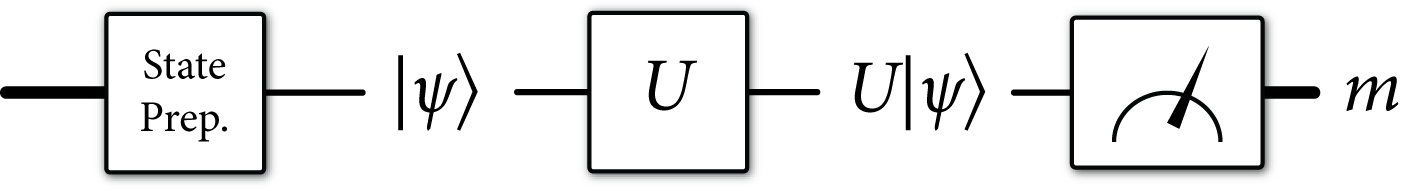
\includegraphics[width=\textwidth]{images/quantum-information-process.png}	
	\end{center}
}

\frame{
	\frametitle{Quantum Gates}
	
	\begin{block}{Hadamard Gate}
		\begin{columns}
  			\column{.5\textwidth}    		
				\begin{align*}
					H &\equiv \ket{+} \bra{0} + \ket{-} \bra{1} \\
					&= \frac{1}{\sqrt{2}}
					\begin{bmatrix}
					 	1 & 1 \\
					 	1 & -1
					\end{bmatrix}			 
				\end{align*}
  			\column{.5\textwidth}
  				\begin{align*}
					H \ket{0} &\longrightarrow \ket{+} \\
					H \ket{1} &\longrightarrow \ket{-} \\
				\end{align*}
		\end{columns}
	\end{block}
	
	\begin{block}{Controlled Gate}
		\textbf{Controlled-NOT (CNOT) Gate}
		\[
			\alpha \ket{00} + \beta \ket{01} + \gamma \ket{10} + \delta \ket{11} 
			\quad \underrightarrow{\text{CNOT}} \quad 
			\alpha \ket{00} + \beta \ket{01} + \gamma \ket{11} + \delta \ket{10}
		\]
		
		This gate is called \textbf{Controlled-U} gate, if we apply another Unitary operator
		instead of NOT operator
	\end{block}
}

\frame{
	\frametitle{Cloning}
	
	\begin{block}{No Cloning Theorem}
		It is impossible to build a \textbf{Universal Copier}
		of quantum states
	\end{block}
	
	\begin{corollary}
		It is impossible to copy quantum informations, except in two following case:
		\begin{enumerate}
			\item{
				Two states are the same ($\braket{\psi}{\phi} = 1$)
			}
			
			\item{
				Two states are orthogonal ($\braket{\psi}{\phi} = 0$)
			}
		\end{enumerate}
	\end{corollary}
}

\frame{
	\frametitle{Entanglement}
	
	\begin{block}{Finding Qubit State!}
		Suppose Alice and Bob shared following two states:
		\begin{align*}
			\ket{0}^A \ket{1}^B \rightarrow 
			&\left\{
			\begin{array}{lc}
				\mbox{Alice Qubit State: } & \ket{0}^A \\
				\mbox{Bob Qubit State: } & \ket{1}^B 
			\end{array}
			\right.
			\\
			\ket{\Phi^+}^{AB} = \frac{\ket{0}^A \ket{0}^B + \ket{1}^A \ket{1}^B}{\sqrt{2}} \rightarrow 
			&\left\{
			\begin{array}{lc}
				\mbox{Alice Qubit State: } & ? \\
				\mbox{Bob Qubit State: } & ? 
			\end{array}
			\right.			
		\end{align*}
		
%		The second state is called an \textbf{Entanglement} state
	\end{block}
	
	\begin{example}{Entanglement States (Bell States)}
		\begin{align*}
			\ket{\Phi^+}^{AB} &\equiv \frac{1}{\sqrt{2}} \left( \ket{00}^{AB} + \ket{11}^{AB} \right) & \quad
			\ket{\Phi^-}^{AB} &\equiv \frac{1}{\sqrt{2}} \left( \ket{00}^{AB} - \ket{11}^{AB} \right) & \\
			\ket{\Psi^+}^{AB} &\equiv \frac{1}{\sqrt{2}} \left( \ket{01}^{AB} + \ket{10}^{AB} \right) & \quad
			\ket{\Psi^-}^{AB} &\equiv \frac{1}{\sqrt{2}} \left( \ket{01}^{AB} - \ket{10}^{AB} \right)
		\end{align*}
	\end{example}
}

\frame{
	\frametitle{Noisy Quantum State}
	
	\begin{block}{Density Operator}
		Suppose we want to perform measurement $\left\{ \Pi_j \right\}$ on system 
		$\mathcal{E} = \left\{ p_X(x), \ket{\psi_x} \right\}_{x \in \mathcal{X}}$. If system is in 
		state $\ket{\psi_x}$, we have
		\begin{align*}
			p_{J|X}(j|x) &= \bra{\psi_x}\Pi_j\ket{\psi_x} \\
			p_J(j) &= \sum_{x \in \mathcal{X}}  p_{J|X}(j|x) p_X(x) \\
			&= \sum_{x \in \mathcal{X}} \bra{\psi_x}\Pi_j\ket{\psi_x} p_X(x) \\
			&= \Tr \left\{ \Pi_j \sum_{x \in \mathcal{X}} p_X(x) \ket{\psi_x} \bra{\psi_x} \right\} \\
			&= \Tr \left\{ \Pi_j \rho \right\}
		\end{align*}
		
		$\rho = \sum_{x \in \mathcal{X}} p_X(x) \ket{\psi_x} \bra{\psi_x}$ 
		is called \textbf{Density Operator}
	\end{block}
}

\frame{
	\frametitle{Properties}
	
	\begin{block}{Properties of Density Operator}
		\begin{enumerate}
			\item{
				$\Tr\{\rho\} = 1$
			}
			
			\item{
				$\rho \geq 0 \quad \bra{\phi} \rho \ket{\phi} \geq 0 \quad \forall \ket{\phi} $
			}
			
			\item{
				$\rho^\dag = \rho$
			}
		\end{enumerate}
	\end{block}
	
	\begin{alertblock}{Note}
		Sate of a quantum system is in fact a density operator		
	\end{alertblock}
}

\frame{
	\frametitle{Noisy Quantum Measurement}
	
	\begin{block}{Measurement}
		The most general quantum measurement, consists of a set of measurement operators
		$\left\{ M_j \right\}_j$, where $\sum_j M_j^\dag M_j = I$.
		
		The probability for obtaining outcome $j$ on quantum state $\rho$ is
		\[
			p(j) = \Tr \left\{ M_j^\dag M_j \rho \right\}
		\]
	\end{block}
	
	\begin{block}{Positive Operator-Valued Measurement (POVM)}
		\textbf{POVM} is a set of measurement operators $\left\{ \Lambda_j \right\}_j$,
		that satisfies following conditions:
		\begin{enumerate}
			\item{
				$\Lambda_j \geq 0$
			}
			
			\item{
				$\sum_j \Lambda_j = I$
			}
		\end{enumerate}
		The probability of outcome $j$ for some density operator $\rho$ is: $\Tr\left\{ \Lambda_j \rho \right\}$		
	\end{block}
}

\frame{
	\frametitle{Ensemble of an Ensemble}
	
	\begin{block}{Classical-Quantum Ensemble}
		\textbf{Problem:} If Alice prepares following ensemble
		\[
			\left\{ p_X(x), \rho_x \right\}_{x \in \mathcal{X}}, \quad \rho = \sum_{x \in \mathcal{X}} p_X(x) \rho_x
		\]
		Bob can't learn about random variable $X$, because there is loss of information in the random variable $X$
		
		\textbf{Solution:}
		\[
			\left\{ p_X(x), \ket{x}\bra{x}^X \otimes \rho_x^A \right\}_{x \in \mathcal{X}}, \quad
			\rho^{XA} = \sum_{x \in \mathcal{X}} p_X(x) \ket{x} \bra{x}^X \otimes \rho_x^A
		\]
	\end{block}
}

\frame{
	\frametitle{Purified State}
	
	\begin{block}{Purification}
		Suppose we are given density operator $\rho^A = \sum_x p_X(x) \ket{x} \bra{x}^A$
		
		Purification of $\rho^A$ is
		\[
			\ket{\psi}^{RA} = \sum_x \sqrt{p_X(x)} \ket{x}^R \ket{x}^A
		\]
		where
		\[
			\rho^A = \Tr_R \left\{ \ket{\psi} \bra{\psi}^{RA} \right\}
		\]
	\end{block}
}

\section{Quantum Information Theory}

\frame{
	\frametitle{Quantum Entropies}
	
	\begin{block}{Von Neumann Entropy}
		\begin{align*}
			H(\rho) &= - \Tr (\rho \log \rho) \\
			&= - \sum_x \lambda_x \log \lambda_x
		\end{align*}	
	\end{block}
	
	\begin{block}{Quantum Joint Entropy}
		\[
			H(AB) = - \Tr \left( \rho^{AB} \log \rho^{AB} \right)
		\]
	\end{block}
	
	\begin{block}{Quantum Conditional Entropy}
		\[
			H(A|B) = H(AB) - H(B)
		\]
	\end{block}
}

\frame{
	\frametitle{Properties}
	
	\begin{block}{Properties of Von Neumann Entropy}
		\begin{enumerate}
			\item{
				$H(\rho) \geq 0$
			}
			
			\item{
				$H(\rho) \leq \log d$ (in $d$-dimensional Hilbert space)
			}
			
			\item{
				For a \textbf{pure} composite system like $AB$: $H(A) = H(B)$
			}
			
			\item{
				$H \left( \sum_i p_i \rho_i \right) = H(p_i) + \sum_i p_i H(\rho_i)$
			}
			
			\item{
				(\textbf{Joint Entropy Theorem}) 
				$H \left( \sum_i p_i |i\rangle \langle i| \otimes \rho_i \right) = H(p_i) + \sum_i p_i H(\rho_i)$
			}
		\end{enumerate}
	\end{block}
}

\frame{
	\frametitle{Quantum Informations}
	
	\begin{block}{Quantum Mutual Information}
		\begin{align*}
			I(A; B) &\equiv H(A) + H(B) - H(AB) \\
			&= H(A) - H(A | B) \\
			&= H(B) - H(B | A)
		\end{align*}
	\end{block}
	
	\begin{block}{Conditional Quantum Mutual Information}
		\[
			I(A; B | C)_\rho \equiv H(A | C)_\rho + H(B | C)_\rho - H(AB | C)_\rho
		\]
	\end{block}
	
	\begin{block}{Coherent Information}
		\[
			I(A\rangle B) = H(‌B) - H(AB)
		\]
	\end{block}
}

\frame{
	\frametitle{Von Neumann Entropy}
	
	\begin{block}{Additivity}
		\[
			H(\rho \otimes \sigma) = H(\rho) + H(\sigma)
		\]
	\end{block}
	
	\begin{block}{Subadditivity \& Triangle Inequality}
		\begin{align*}
			H(\rho^{AB}) &\leq  H(\rho^{A}) + H(\rho^{B}) &\mbox{Subadditivity Inequality}\\
			H(\rho^{AB}) &\geq  \abs{H(\rho^{A}) - H(\rho^{B})} &\mbox{Triangle Inequality}
		\end{align*}
	\end{block}
	
	\begin{block}{Concavity of Von Neumann Entropy}
		\[
			H \left( \sum_i p_i \rho_i \right) \geq \sum_i p_i H(\rho_i)
		\]
	\end{block}
}

\section{Quantum Channels}

\frame{
	\frametitle{Classical Channel}
	
	\begin{block}{Communication System}		
		\begin{center}
			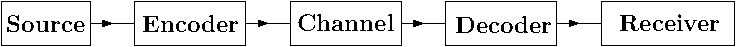
\includegraphics[width=\textwidth]{images/communication-system.png}	
		\end{center}
	\end{block}
}

\frame{
	\frametitle{Random Operator}
	
	\begin{block}{Random Unitary Operator}
		By applying ensemble of unitaries, $\left\{ p(k), U_k \right\}_{k \in \mathcal{K}}$ to 
		an ensemble of state, $\left\{ p_X(x), \ket{\psi_x} \right\}_{x \in \mathcal{X}}$,
		we obtain following density operator
		\[
			\sum_{k \in \mathcal{K}} p(k) U_k \rho U_k^\dag
		\]
		where
		\[
			\rho = \sum_{x \in \mathcal{X}} p_X(x) \ket{\psi_x} \bra{\psi_x}
		\]
	\end{block}
}

\frame{
	\frametitle{Noisy Evolution}
	
	\begin{block}{Quantum Channel}
		\textbf{Ensemble of states:} $\left\{ p_X(x), \ket{\psi_x} \right\}$
		
		\textbf{Measurement operators:} $\{ M_k \}$ where $\sum_k M_k^\dag M_k = I$
		
		\begin{itemize}
			\item{
				Probability of outcome $k$ where state is $\ket{\psi_x}$:
				\begin{center}
					$p_{K|X}(k|x) = \bra{\psi_x} M_k^\dag M_k \ket{\psi_x}$
				\end{center}
			}
			
			\item{
				If we loss track of measurement outcome, for resulting ensemble description we have
				\[
					\left\{ p_{X \vert K}(x \vert k) p_K(k), \frac{M_k \ket{\psi_x}}{\sqrt{p_{K \vert X}(k \vert x)}} \right\}					
				\]
				and its density operator is
				\[
					\sum_{x, k} p_{X \vert K}(x \vert k) p_K(k) \frac{M_k \ket{\psi_x} \bra{\psi_x} M_k^\dag}{p_{K \vert X}(k \vert x)}
					= \sum_k M_k \rho M_k^\dag
				\]
			}
		\end{itemize}
	\end{block}
}

\frame{
	\frametitle{Noisy Evolution (Cont.)}
	
	\begin{block}{Result}
		We can summarize the whole operations as a noisy map:
		\[
			\mathcal{N}(\rho) = \sum_k M_k \rho M_k^\dag
		\]
	\end{block}

	\vspace*{10pt}	
	
	\begin{center}
		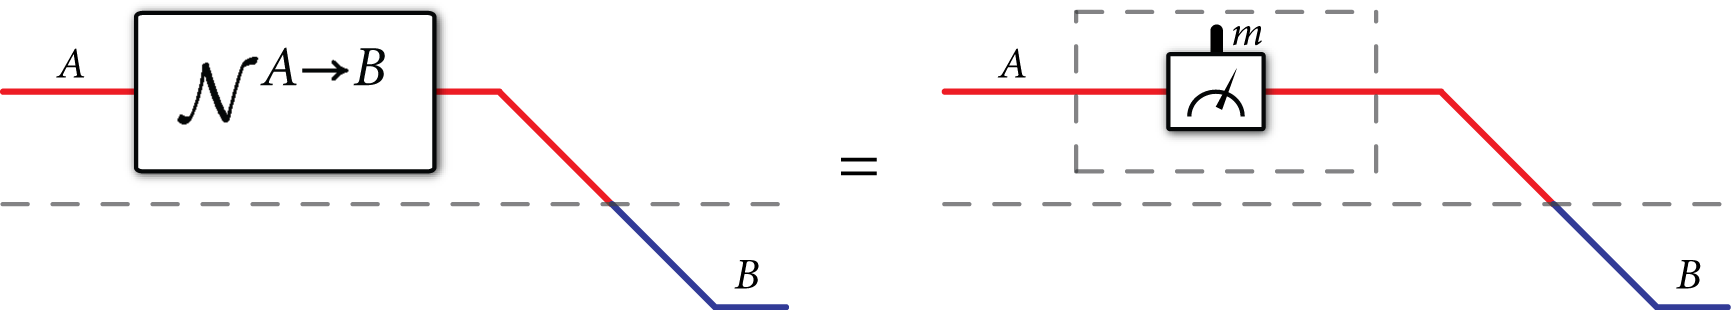
\includegraphics[width=\textwidth]{images/noisy-quantum-channel.png}	
	\end{center}
}

\frame{
	\frametitle{Examples of Noisy Quantum Channels}	
	
	\begin{block}{Depolarizing Channel}
		\[
			\rho \longrightarrow (1 - p) \rho + p \pi
		\]
	\end{block}
	
	\begin{block}{Erasure Channel}
		\[
			\rho \longrightarrow (1 - \varepsilon) \rho + \varepsilon \ket{e} \bra{e}
		\]
	\end{block}
}

%\frame{
%	\frametitle{Examples of Noisy Quantum Channels (Cont.)}
%	
%	\begin{block}{Classical-Quantum (Entanglement-Breaking) Channel}
%		\textbf{Channel input:} Density operator $\rho$ which acts on orthonormal basis $\{ \ket{k} \}_k$ 
%	
%		\textbf{Process:}
%		\begin{enumerate}
%			\item{
%				Performs measurement in basis $\ket{k}$ $\rightarrow$ Post measurement state:
%				\[
%					\frac{\ket{k} \bra{k} \rho \ket{k} \bra{k}}{\bra{k} \rho \ket{k}}
%				\]
%			}
%		
%			\item{
%				Correlates a density operator $\sigma_k$ with the post measurement state. That leads to
%				following ensemble and density operator
%				\[
%					\left\{ \bra{k} \rho \ket{k}, \frac{\ket{k} \bra{k} \rho \ket{k} \bra{k}}{\bra{k} \rho \ket{k}} 
%					\otimes \sigma_k \right\}
%				\]			
%				\[
%					\sum_k \ket{k} \bra{k} \rho \ket{k} \bra{k} \otimes \sigma_k
%				\]
%		}
%	\end{enumerate}
%	\end{block}
%}
%
%\frame{
%	\frametitle{Examples of Noisy Quantum Channels (Cont.)}
%	
%	\begin{block}{Classical-Quantum (Entanglement-Breaking) Channel (Cont.)}
%		Then channel outputs the second system
%		\[
%			\mathcal{N}(\rho) = \sum_k \bra{k} \rho \ket{k} \sigma_k
%		\]
%	\end{block}
%
%	\vspace*{10pt}	
%	
%	\begin{center}
%		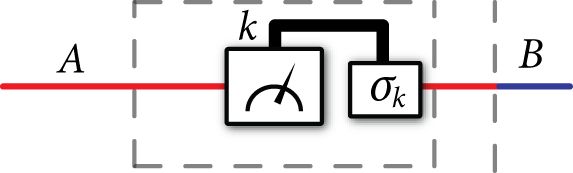
\includegraphics[width=.6\textwidth]{images/classical-quantum-channel.png}	
%	\end{center}
%}

\frame{
	\frametitle{Data Processing}
	
	\begin{block}{Quantum Data Processing Inequality}
		Suppose Alice and Bob share state $\ket{\phi}^{AB}$, then
		\[
			I(A \rangle B)_\phi \geq I(A \rangle B_1)_\rho \geq I(A \rangle B_2)_\sigma
		\]
		where
		\begin{align*}
			\rho^{AB_1} &\equiv \mathcal{N}_1^{B \rightarrow B_1}\left(\phi^{AB}\right) \\
			\sigma^{AB_2} &\equiv \mathcal{N}_2^{B_1 \rightarrow B_2}\left(\rho^{AB_1}\right)			
		\end{align*}
	\end{block}
	
	\begin{center}
		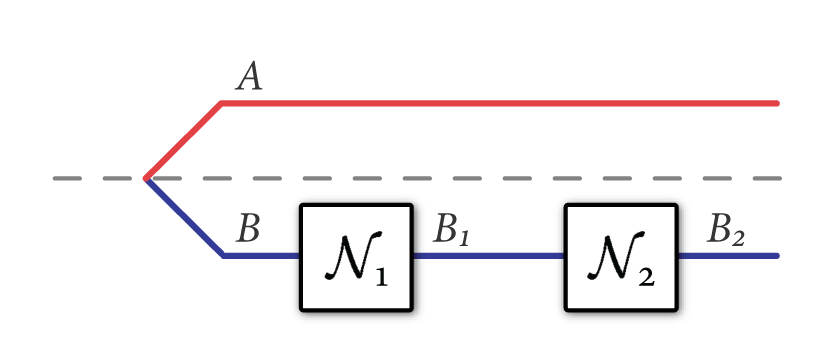
\includegraphics[width=.6\textwidth]{images/quantum-data-processing.png}	
	\end{center}
}

\frame{
	\frametitle{Quantum Channel Informations}
	
	\begin{block}{Holevo Information of Quantum Channel}
		\[
			\chi (\mathcal{N}) \equiv \max_{\rho^{XA^\prime}} I(X; B)_\rho
		\]
		where
		\begin{align*}
			\rho^{XA^\prime} &\equiv \sum_x p_X(x) \ket{x} \bra{x}^X \otimes \rho_x^{A^\prime} \\
			\rho^{XB} &\equiv \sum_x p_X(x) \ket{x} \bra{x}^X \otimes \mathcal{N}^{A^\prime \rightarrow B} \left( \rho_x^{A^\prime} \right)
		\end{align*}
	\end{block}
}

\frame{
	\frametitle{Quantum Channel Informations (Cont.)}
	
	\begin{block}{Additivity of Holevo Information}
		\[
			\chi \left(\mathcal{N}_1 \otimes \mathcal{N}_2 \right) = \chi \left(\mathcal{N}_1 \right) + \chi \left( \mathcal{N}_2 \right)
		\]
		where $\mathcal{N}_1$ and $\mathcal{N}_2$ are \textbf{Entanglement-Breaking} channels
	\end{block}

	\begin{center}
		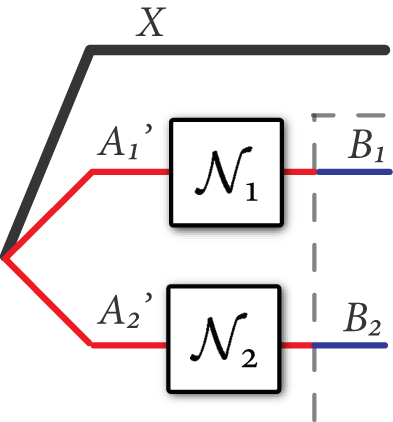
\includegraphics[width=.3\textwidth]{images/additivity-holevo-figure.png}	
	\end{center}
}

\frame{
	\frametitle{Quantum Channel Informations (Cont.)}
	
	\begin{block}{Mutual Information of Quantum Channel}
		\[
			I(\mathcal{N}) \equiv \max_{\phi^{AA^\prime}} I(A; B)_{\rho^{AB}}
		\]
		where
		\[
			\rho^{AB} = \mathcal{N}^{A^\prime \rightarrow B} (\phi^{AA^\prime})
		\]
	\end{block}
	
	\begin{block}{Additivity of Mutual Information}
		\[
			I \left(\mathcal{N}_1 \otimes \mathcal{N}_2 \right) = I \left(\mathcal{N}_1 \right) + I \left( \mathcal{N}_2 \right)
		\]
	\end{block}
}

\frame{
	\frametitle{Quantum Channel Informations (Cont.)}
	
	\begin{block}{Coherent Information of Quantum Channel}
		\[
			Q(\mathcal{N}) \equiv \max_{\phi^{AA^\prime}} I(A\rangle B)_\rho
		\]
		where
		\[
			\rho^{AB} = \mathcal{N}^{A^\prime \rightarrow B} (\phi^{AA^\prime})
		\]
	\end{block}
	
	\begin{block}{Additivity of Coherent Information}
		\[
			Q(\mathcal{N}_1 \otimes \mathcal{N}_2) = Q(\mathcal{N}_1) + Q(\mathcal{N}_2)
		\]
		where $\mathcal{N}_1$ and $\mathcal{N}_2$ are \textbf{Degradable} channels
	\end{block}	
}

\frame{
	\frametitle{Quantum Channel Informations (Cont.)}
	
	\begin{block}{Private Information of Quantum Channel}
		\[
			P(\mathcal{N}) \equiv \max_{\rho^{XA^\prime}} \left\{ I(X; B)_\rho - I(X; E)_\rho \right\}
		\]
		where
		\begin{align*}
			\rho^{XA^\prime} &= \sum_x p_X(x) \ket{x} \bra{x}^X \otimes \rho_x^{A^\prime} \\
			\rho^{XBE} &= \sum_x p_X(x) \ket{x} \bra{x}^X \otimes U_{\mathcal{N}}^{A^\prime \rightarrow BE} \left( \rho_x^{A^\prime} \right)
		\end{align*}
	\end{block}
	
	\begin{block}{Private and Coherent Information of Quantum Channel Relation}
		\[
			Q(\mathcal{N}) \leq P(\mathcal{N})
		\]
	\end{block}	
}

\frame{
	\frametitle{Quantum Channel Informations (Cont.)}
	
	\begin{block}{Additivity of Private Information}
		\[
			P \left(\mathcal{N}_1 \otimes \mathcal{N}_2 \right) = P \left(\mathcal{N}_1 \right) + P \left( \mathcal{N}_2 \right)
		\]
		where $\mathcal{N}_1$ and $\mathcal{N}_2$ are \textbf{Degradable} channels
	\end{block}

	\begin{center}
		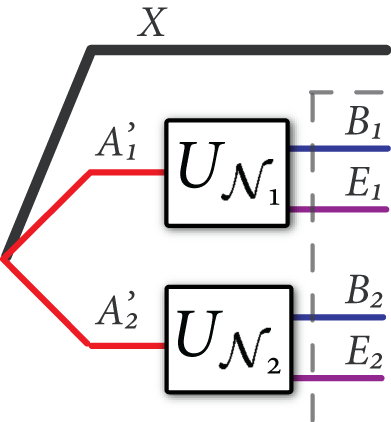
\includegraphics[width=.3\textwidth]{images/additivity-private.png}	
	\end{center}
}

\section{Channel Capacity and Additivity Violation}

\frame{
	\frametitle{Classical Channel}
	
	\begin{block}{Capacity of Classical Channel}
		\[
			C(\mathcal{N}) = \max_X I(X; Y)
		\]
	\end{block}
	
	\begin{block}{Additivity of Classical Channel}
		\[
			C \left(\mathcal{N}_1 \otimes \mathcal{N}_2 \right) = C \left(\mathcal{N}_1 \right) + C \left( \mathcal{N}_2 \right)
		\]
	\end{block}
}

\frame{
	\frametitle{Overview of Quantum Channel}
	
	\begin{center}
		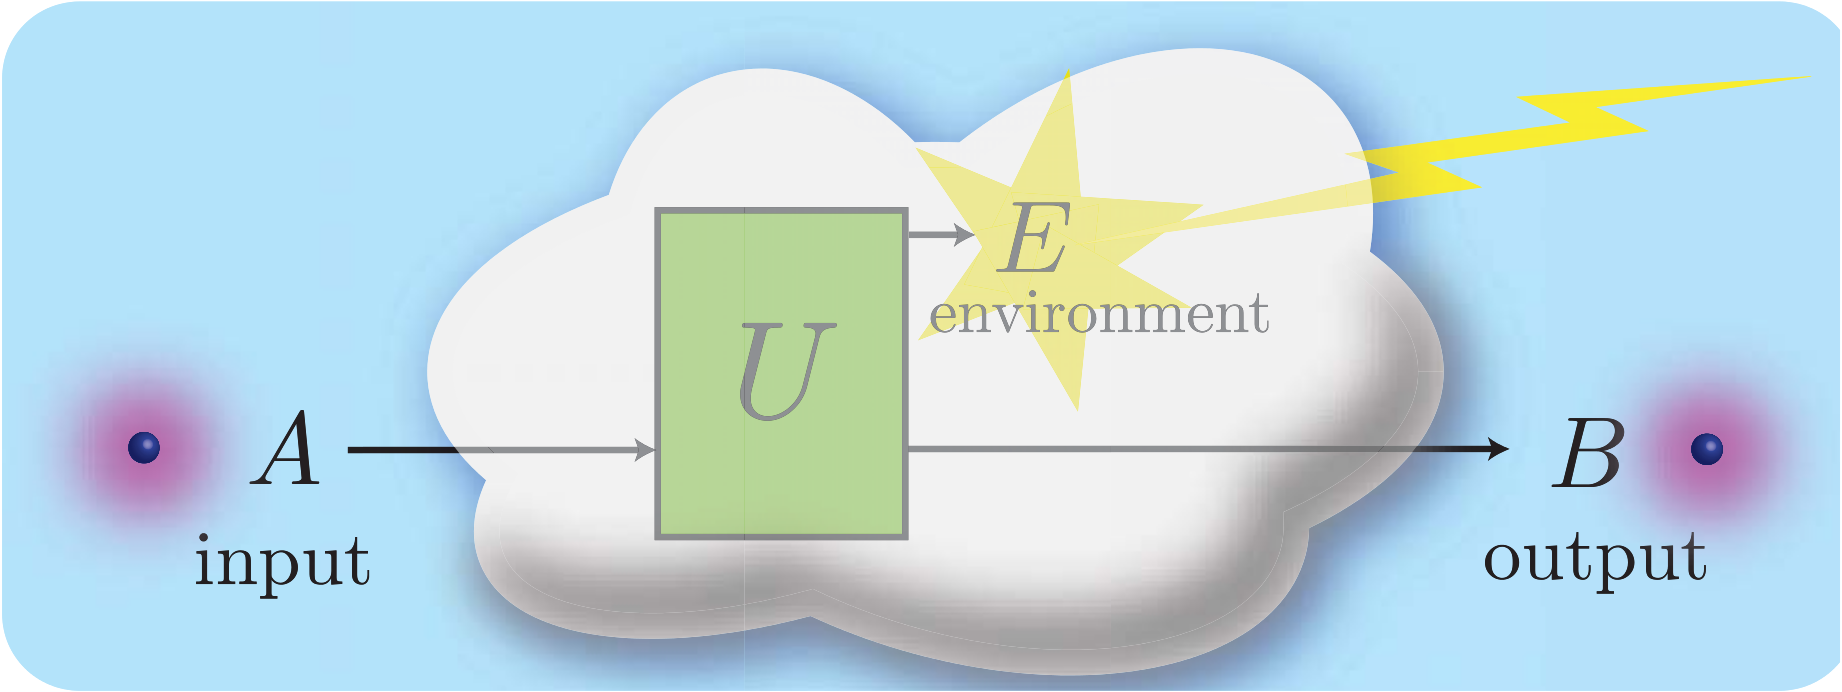
\includegraphics[width=\textwidth]{images/quantum-channel-representation.png}	
	\end{center}
}

\frame{
	\frametitle{Quantum Channel Capacities}
	
	\begin{block}{Quantum Capacity of Quantum Channel}
		\[
			Q(\mathcal{N}) = \lim_{n \rightarrow \infty} \frac{1}{n} Q^{(1)} \left(\mathcal{N}^{\otimes n}\right)
		\]
		where
		\[
			Q^{(1)} = \max_{\rho^A} \left(H(B) - H(E)\right)
		\]
	\end{block}
	
	\begin{center}
		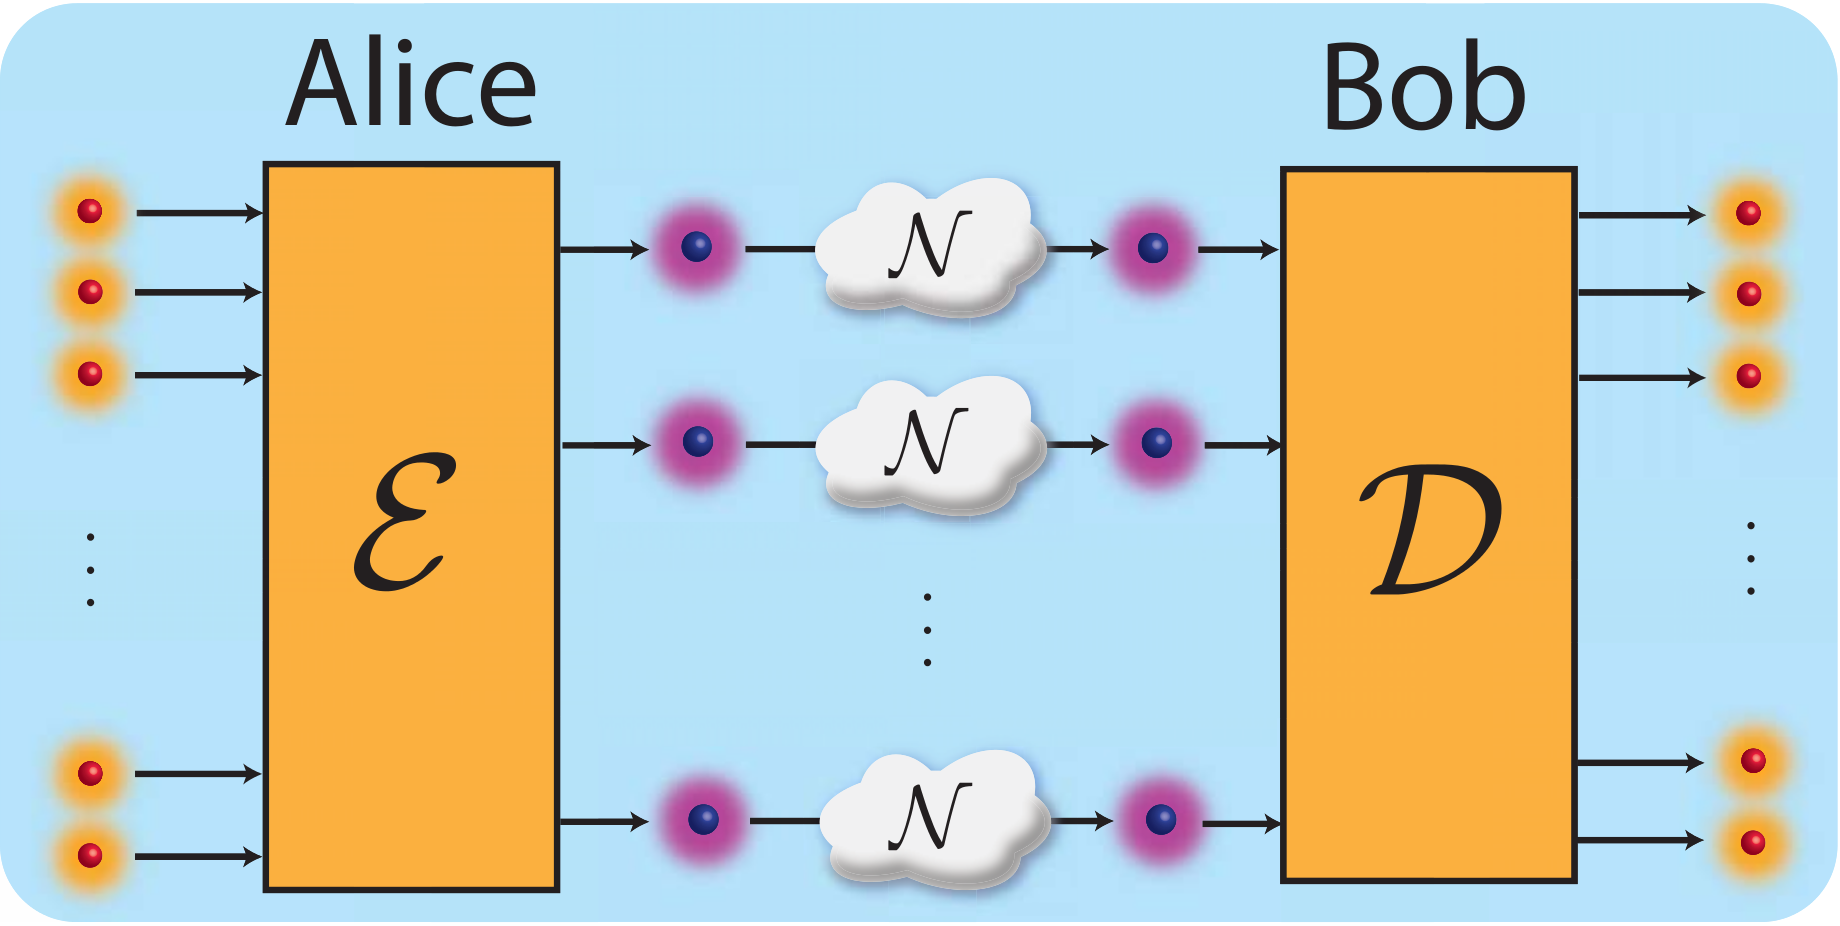
\includegraphics[width=.75\textwidth]{images/quantum-channel-quantum-capacity.png}	
	\end{center}
}

\frame{
	\frametitle{Quantum Channel Capacities (Cont.)}
	
	\begin{block}{Private Capacity of Quantum Channel}
		\[
			P(\mathcal{N}) = \lim_{n \rightarrow \infty} \frac{1}{n} P^{(1)} \left(\mathcal{N}^{\otimes n}\right)
		\]
		where
		\[
			P^{(1)} = \max_{X, \rho_x^A} \left(I(X; B) - I(X; E)\right)
		\]
	\end{block}
}

\frame{
	\frametitle{Private Capacity of Quantum Channel is not Additive}
	
	\begin{block}{Introduction}
		A quantum channel $\mathcal{N}$ is described by an isometric map $V: A \rightarrow BE$,
		\[
			\mathcal{N}(\rho) = \Tr_E\left(V \rho V^\dag\right), \quad \quad 
			\widetilde{\mathcal{N}}(\rho) = \Tr_B\left(V \rho V^\dag\right)
		\]		
	\end{block}
	
	\begin{block}{Quantum Channel Capacities Relation}
		\[
			C(\mathcal{N}) \geq P(\mathcal{N}) \geq Q(\mathcal{N})			
		\]
		where
		\begin{align*}
			\chi (\mathcal{N}) &\leq C(\mathcal{N}) 
			= \lim_{n \rightarrow \infty} \frac{1}{n} \chi \left( \mathcal{N}^{\otimes n} \right)\\
			P^{(1)}(\mathcal{N}) &\leq P(\mathcal{N}) 
			= \lim_{n \rightarrow \infty} \frac{1}{n} P^{(1)} \left( \mathcal{N}^{\otimes n} \right)\\
			Q^{(1)} (\mathcal{N}) &\leq Q(\mathcal{N}) 
			= \lim_{n \rightarrow \infty} \frac{1}{n} Q^{(1)} \left( \mathcal{N}^{\otimes n} \right)
		\end{align*}
	\end{block}
}

\frame{
	\frametitle{Channel Construction ($\mathcal{T}_{\mathcal{N}}^k$)} 
	
	\begin{center}
		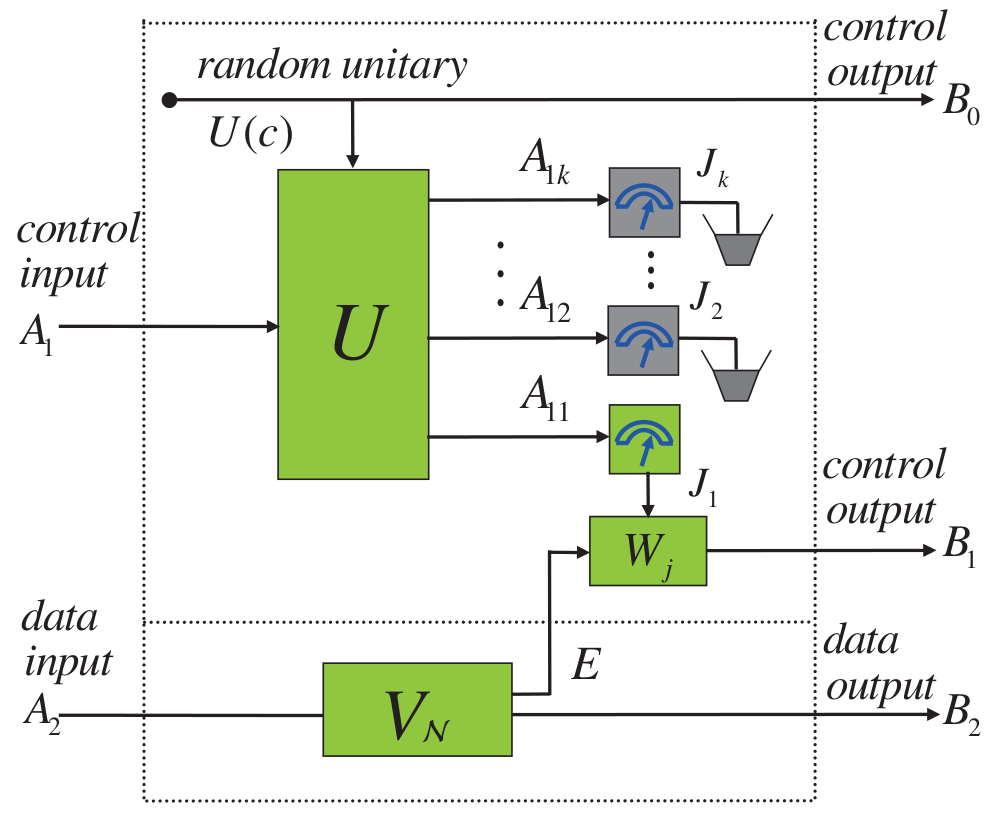
\includegraphics[width=.75\textwidth]{images/constructed-channel.png}	
	\end{center}
}

\frame{
	\frametitle{Private Capacity of Quantum Channel is not Additive (Cont.)}
	
	\begin{theorem}
		For any channel $\mathcal{N}$ with input space $A$, output space $B$ and
		environment $E$ and any integer $k$, let
		$\delta(k) = \frac{1}{k} \left( 5 + 4 \log \abs{E} \right)$, then for arbitrary channel
		$\mathcal{E}$,
		\[
			\chi(\mathcal{N} \otimes \mathcal{E}) \leq \chi \left( \mathcal{T}_\mathcal{N}^k \otimes \mathcal{E} \right)
			\leq \chi (\mathcal{N} \otimes \mathcal{E}) + \delta(k)
		\]
		As a consequence
		\[
			C(\mathcal{N}) \leq C\left(\mathcal{T}_\mathcal{N}^k\right) \leq C(\mathcal{N}) + \delta(k)
		\]
	\end{theorem}
}

\frame{
	\frametitle{Private Capacity of Quantum Channel is not Additive (Cont.)}
	
	\begin{block}{Additivity Violation}
		If Alice prepare a maximally entangled state $\Phi$ and another arbitrary state $\rho$,
		then feeds them to channel $\mathcal{T}_\mathcal{N}^k \otimes \mathcal{A}$,
		where $\mathcal{A}$ is 50\% erasure channel, we have
		\[
			P\left(\mathcal{T}_\mathcal{N}^k \otimes \mathcal{A}\right) \geq 
			Q\left(\mathcal{T}_\mathcal{N}^k \otimes \mathcal{A}\right) \geq 
			Q_E(\mathcal{N})
		\]
		where
		\begin{align*}
			Q_E(\mathcal{N}) &= \max_\rho I_c\left(\Phi \otimes \rho, \mathcal{T}_\mathcal{N}^k \otimes \mathcal{A}\right) \\
			Q_E(\mathcal{N}) &> C(\mathcal{N})
		\end{align*}
		
		So for sufficiently larg $k$,
		\[
			P\left(\mathcal{T}_\mathcal{N}^k \otimes \mathcal{A}\right) \geq 
			Q\left(\mathcal{T}_\mathcal{N}^k \otimes \mathcal{A}\right) >
			P\left(\mathcal{T}_\mathcal{N}^k\right) \geq
			Q\left(\mathcal{T}_\mathcal{N}^k\right)
		\]
	\end{block}
}

\frame{
	\frametitle{Private Capacity of Quantum Channel is not Additive (Cont.)}
	
	\begin{block}{Conclusion}
		We showed a way of converting any gap between channel classical capacity and
		entanglement-assisted capacity into the violation of the additivity of the private
		capacity of the channel tensored with 50\% erasure channel
	\end{block}
}

\frame{
	\frametitle{References}
	
	\begin{thebibliography}{1}
		\bibitem{ref1}[Quantum Computation and Quantum Information]
		\newblock Nielsen, Michael A. and Isaac, L. Chuang
		\newblock Cambridge University Press (September 2000)
	\end{thebibliography}
	
	\begin{thebibliography}{2}
		\bibitem{ref2}[From Classical to Quantum Shanon Theory]
		\newblock Mark M. Wilde
		\newblock School of Computer Science McGill University (June 2011)
	\end{thebibliography}
	
	\begin{thebibliography}{3}
		\bibitem{ref3}[Private Capacity of Quantum Channels is Not Additive]
		\newblock K. Li, A. Winter, X. Zou, GC. Guo
		\newblock Phys. Rev. Lett. 103:120501 (2009)
	\end{thebibliography}
	
	\begin{thebibliography}{4}
		\bibitem{ref4}[Quantum Communication With Zero-Capacity Channels]
		\newblock G. Smith, J. Yard
		\newblock Science 321:1812 (2008)
	\end{thebibliography}
	
	\begin{thebibliography}{5}
		\bibitem{ref5}[The Capacity of the Quantum Channel With General Signal States]
		\newblock A. S. Holevo
		\newblock IEEE Trans. Info. Theory 44:269 (1998)
	\end{thebibliography}	
}

\frame{
	\frametitle{References (Cont.)}
	
	\begin{thebibliography}{6}
		\bibitem{ref6}[Sending Classical Information via Noisy Quantum Channels]
		\newblock B. Schumacher, M. D. Westmorland
		\newblock Phys. Rev. A 56:131 (1997)
	\end{thebibliography}
	
	\begin{thebibliography}{7}
		\bibitem{ref7}[The Private Classical Capacity and Quantum Capacity of a Quantum Channel]
		\newblock I. Devetak
		\newblock IEEE Trans. Info. Theory 51:44 (2005)
	\end{thebibliography}
	
	\begin{thebibliography}{8}
		\bibitem{ref8}[The Capacity of the Noisy Quantum Channel]
		\newblock S. Lloyd
		\newblock Phys. Rev. A 55:1613 (1997)
	\end{thebibliography}
	
	\begin{thebibliography}{9}
		\bibitem{ref9}[Quantum Error Correction]
		\newblock P. W. Shor
		\newblock http://www.msri.org/publications/ln/msri/2002/quantum crypto/shor/1/
	\end{thebibliography}		
}

\frame{
	\begin{center}
		\textbf{\Large{\color{gray}Thanks for your attention}}
	\end{center}
	\vspace*{30pt}
	\begin{flushright}
		\small{\textbf{``I think I can safely say that nobody understands quantum mechanics''}}
		
		\tiny{\textit{Nobel-prize winning physicist} \textbf{Richard Feynman}}
	\end{flushright}
	
}
\end{document}